\documentclass[tikz,border=4pt]{standalone}
\usepackage{amsmath}
\usepackage{tikz}
\usetikzlibrary{arrows.meta,positioning,fit,backgrounds,calc,shapes.geometric,decorations.pathreplacing,patterns}
\usepackage{xcolor}
\renewcommand{\familydefault}{\sfdefault}
\definecolor{cdata}{HTML}{1F5FA8}
\definecolor{cctrl}{HTML}{15796F}
\definecolor{cres}{HTML}{6A4C93}
\definecolor{cgray}{HTML}{5A6570}
\definecolor{cwarn}{HTML}{B4561B}
\tikzset{
  base/.style={rounded corners=1.8pt, line width=0.6pt, align=center, font=\scriptsize, inner sep=3pt, minimum height=8mm, text=black!85},
  data/.style={base, draw=cdata, fill=cdata!9},
  ctrl/.style={base, draw=cctrl, fill=cctrl!9},
  res/.style={base, draw=cres, fill=cres!9},
  art/.style={base, draw=black!65, fill=black!7},
  ext/.style={base, draw=cgray, fill=white, dashed},
  gate/.style={font=\tiny\bfseries, text=cwarn, draw=cwarn, rounded corners=1pt, inner sep=1.6pt, fill=white, line width=0.5pt},
  arr/.style={-{Stealth[length=2.0mm,width=1.5mm]}, line width=0.6pt, draw=cgray!85!black},
  arr2/.style={{Stealth[length=2.0mm,width=1.5mm]}-{Stealth[length=2.0mm,width=1.5mm]}, line width=0.6pt, draw=cgray!85!black},
  darr/.style={-{Stealth[length=2.0mm,width=1.5mm]}, line width=0.6pt, dashed, draw=cgray!85!black},
  lbl/.style={font=\tiny, text=cgray!90!black, inner sep=1pt},
  band/.style={rounded corners=3pt, line width=0.7pt},
}
\newcommand{\dotsep}{\,$\cdot$\,}
\renewcommand{\tiny}{\fontsize{6}{7}\selectfont}

\begin{document}
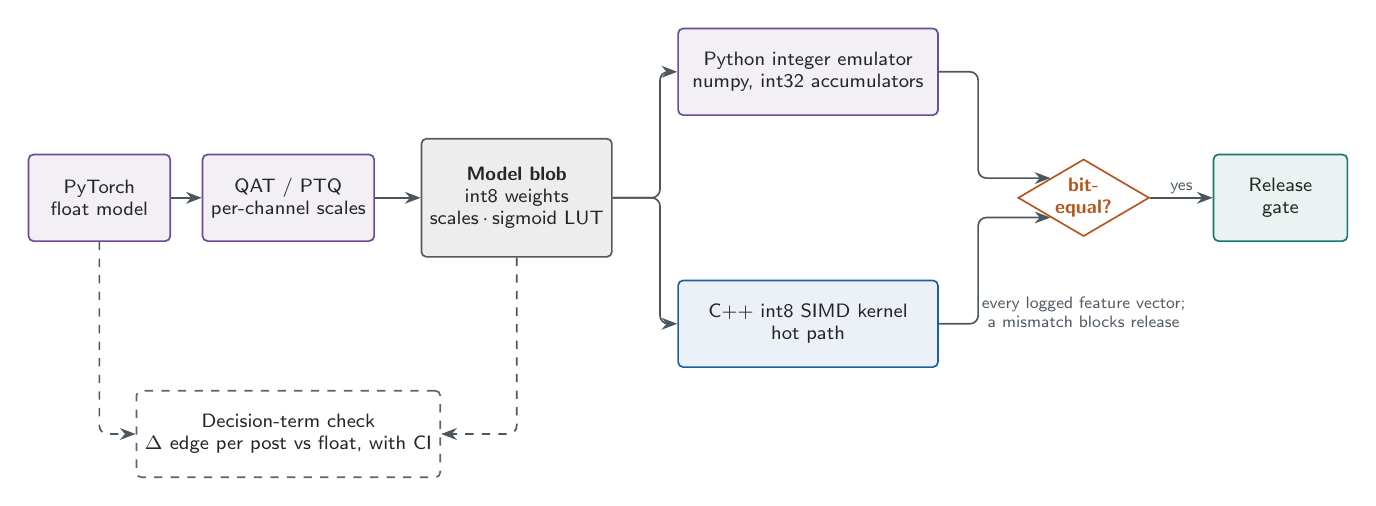
\begin{tikzpicture}
\node[res,  minimum width=1.8cm, minimum height=11mm] (f1) at (1.0,2.0) {PyTorch\\float model};
\node[res,  minimum width=1.9cm, minimum height=11mm] (f2) at (3.4,2.0) {QAT / PTQ\\per-channel scales};
\node[art,  minimum width=2.4cm, minimum height=15mm] (f3) at (6.3,2.0) {\bfseries Model blob\\\normalfont int8 weights\\scales\dotsep sigmoid LUT};
\node[res,  minimum width=3.3cm, minimum height=11mm] (f4) at (10.0,3.6) {Python integer emulator\\numpy, int32 accumulators};
\node[data, minimum width=3.3cm, minimum height=11mm] (f5) at (10.0,0.4) {C++ int8 SIMD kernel\\hot path};
\node[draw=cwarn, diamond, aspect=1.7, fill=white, inner sep=0.5pt, font=\scriptsize\bfseries, text=cwarn, line width=0.6pt, align=center] (f6) at (13.5,2.0) {bit-\\equal?};
\node[ctrl, minimum width=1.7cm, minimum height=11mm] (f7) at (16.0,2.0) {Release\\gate};
\draw[arr] (f1) -- (f2);
\draw[arr] (f2) -- (f3);
\draw[arr, rounded corners=3pt] (f3.east) -- ++(0.6,0) |- (f4.west);
\draw[arr, rounded corners=3pt] (f3.east) -- ++(0.6,0) |- (f5.west);
\draw[arr, rounded corners=3pt] (f4.east) -- ++(0.5,0) |- (f6.north west);
\draw[arr, rounded corners=3pt] (f5.east) -- ++(0.5,0) |- (f6.south west);
\draw[arr] (f6) -- node[above, lbl] {yes} (f7);
\node[lbl, align=center] at (13.5,0.55) {every logged feature vector;\\a mismatch blocks release};
% decision-term check
\node[ext, minimum width=3.6cm, minimum height=11mm] (chk) at (3.4,-1.0) {Decision-term check\\$\Delta$ edge per post vs float, with CI};
\draw[darr, rounded corners=3pt] (f1.south) |- (chk.west);
\draw[darr, rounded corners=3pt] (f3.south) |- (chk.east);
\end{tikzpicture}
\end{document}
